% !TeX spellcheck = en_US
\chapter{Implementation}\label{ch:implementation}

In this chapter, it will be discussed how the different approaches of Ch.~\ref{ch:approach} have been implemented. First, the comparison of HDT and GRP is discussed. Second, improvements for both graph and dictionary compression are presented.

\section{GRP vs HDT}\label{sec:implementationGRPvsHDT}

In this chapter, it will be explained how the comparison between HDT and GRP is implemented.

As has just explained, \GHDT{} can compress a graph that is similar to a hub pattern (few subjects, many objects) very well. So, \CRGraph{HDT} gets higher the further away the graph is from this pattern. The most unfavorable graph structure for \GHDT{} is therefore the authority pattern (see Ch.~\ref{sec:approachStarPattern}).

The task is to create a series of RDF graphs $(G_1,...,G_m)$ that first correspond to the hub pattern and then continue to change in the direction of the authority pattern. That can be done using Alg.~\ref{alg:BuildGraphs}. The first input parameter $steps$ influences how many graphs will be created, as it defines by which amount the number of subjects ($subj$) is increased in every iteration of the while loop. It has to chosen low enough to ensure a smooth transition from the hub to authority pattern. The second parameter $nodesFactor$ influences the amount of nodes of the graphs. Concrete values for the parameter are not important to mention.

\begin{algorithm}
	\caption{BuildGraphs ($steps$, $ nodesFactor$)}\label{alg:BuildGraphs}
	\begin{algorithmic}[1]
		\State $n \leftarrow nodesFactor*steps$ // $n$ is the number of nodes
		\State $subj \leftarrow 1$
		\State $i \leftarrow 1$
		\While{$subj < n$ }
		\State $obj \leftarrow$ $n-subj$ 
		\State $G_i \leftarrow$ build graph with $subj$ subjects and $obj$ objects\label{line:buildgraph}
		\State  $subj\leftarrow subj+steps$
		\State  $i\leftarrow i+1$
		\EndWhile
		\State \Return $(G_1,...,G_m)$
	\end{algorithmic}
\end{algorithm}

\clearpage
Fig.~\ref{fig:star_pattern} illustrates how Alg.~\ref{alg:BuildGraphs} works. All graphs ($G_1$ to $G_m$) have the same number of nodes and edges. That is ensured by Line~\ref{line:buildgraph} in Alg.~\ref{alg:BuildGraphs}. $G_1$ has only one subject connected to all objects. $G_2$ then has two subjects more and correspondingly 2 objects less. This continues until there is only one object that is connected to all subjects ($G_m$). The edges are randomly distributed among the nodes, so that all nodes have a similar degree and each node has at least a degree of one.

\begin{figure}[h]
	\centering
	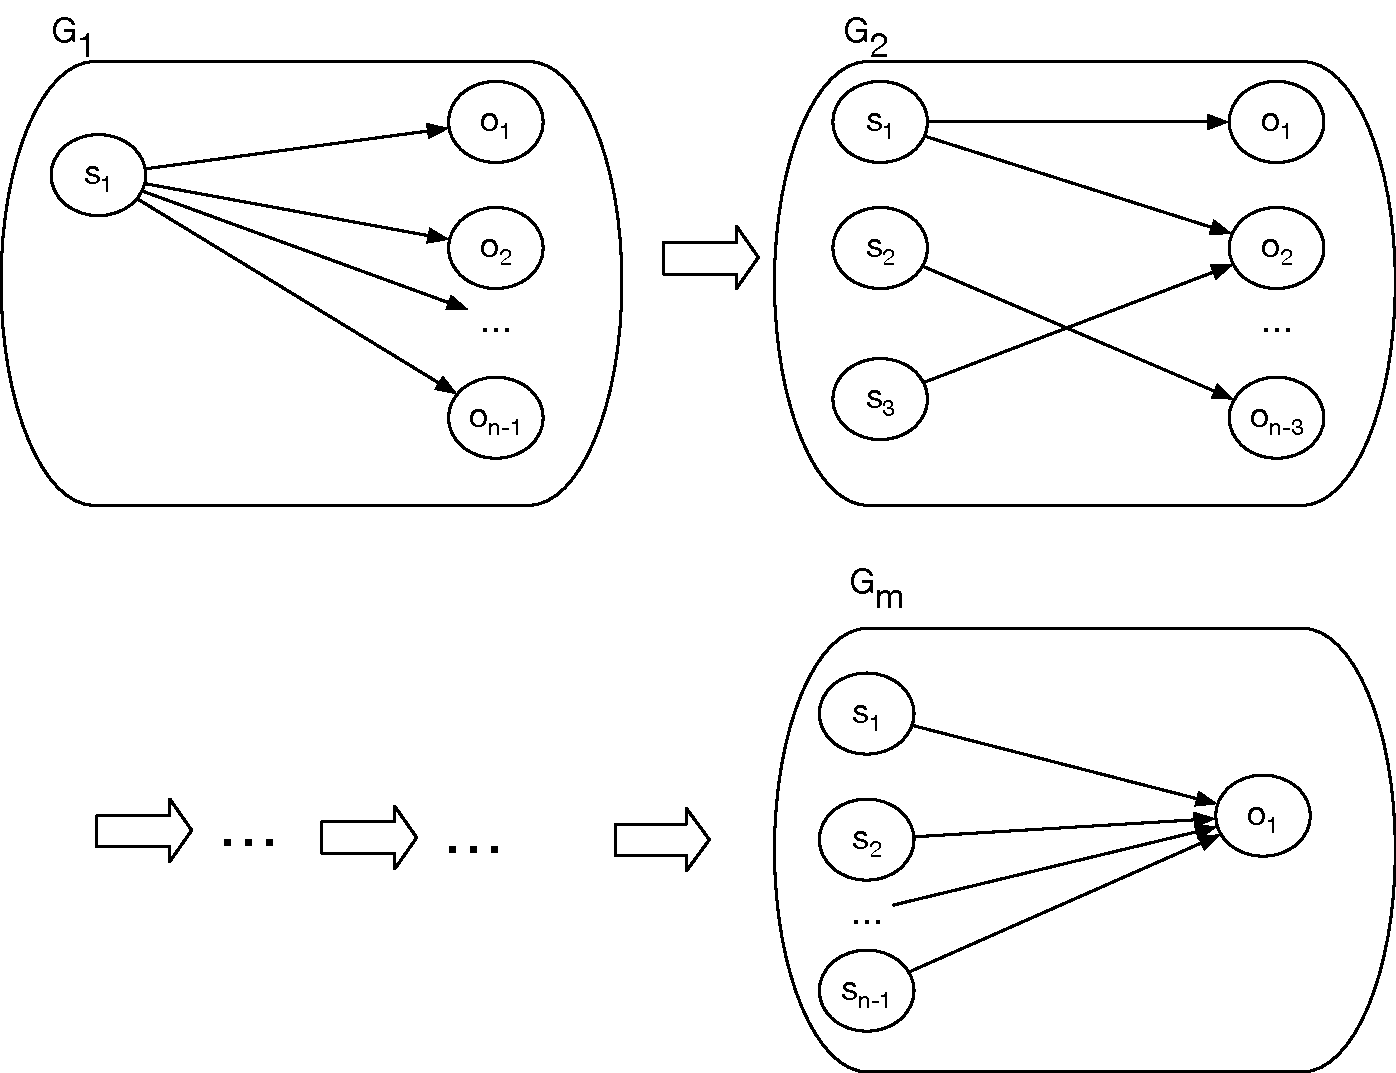
\includegraphics[width=0.8\textwidth]{figures/GRPvsHDT/starpattern.pdf}
	\caption{Illustration of Alg.~\ref{alg:BuildGraphs}: Step-by-step transition from hub pattern to authority pattern. The number of nodes $n$ is the same for each graph. The number of edges is also the same for each graph.}
	\label{fig:star_pattern}
\end{figure}

It is also ensured that each of the generated files has exactly the same size. This is made possible by ensuring that each URI has the same length and that every RDF graph also has the same number of triples. This same size is important for the evaluation, since only the graph's structure is of interest here. An unequal size of the RDF files would lead to undesired effects in terms of $CR_{Graph_C}$.

A section of such a file (for $G_1$) is shown in Fig.~\ref{fig:rdfFile}. In that example, there is only one distinct predicate for all triples. This is because, we first want to focus on the effect of the hub and authority patterns. The impact of an increasing number of predicates will also be evaluated in Ch.~\ref{sec:evaluationHDTvsGRP}.


\begin{figure}[h]
	\centering
	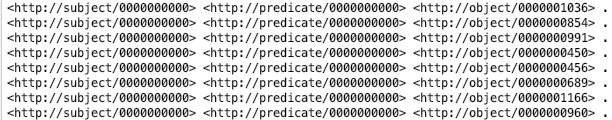
\includegraphics[width=0.8\textwidth]{figures/GRPvsHDT/file.png}
	\caption{Excerpt from the generated RDF file for $G_1$ (see Fig.~\ref{fig:star_pattern}). Each triple has the same length.}
	\label{fig:rdfFile}
\end{figure}

\section{Compression Improvements}\label{sec:implementationComprRatioImprovements}

This chapter introduces the implementation details of Ch.~\ref{sec:approachComprRatioImprovements}. First, applying ontology knowledge in order to achieve a better compression ratio is discussed. Afterwards, implementation details of the dictionary compression improvements are presented.

\subsection{Datasets}\label{sec:implementationDatasets}

Here, an overview of the different datasets, that have been used for the evaluation, is given. Although the datasets are used in Ch.~\ref{ch:evaluation}, they are presented here, since some implementation details are dependent on the data.

\subsubsection{Semantic Web Dog Food}

Semantic Web Dog Food~\footnote{http://www.scholarlydata.org/dumps/} is a collection of RDF files from the Semantic Web community. It contains data about papers, people, organizations, and events of the community. Open source tools are provided for users to contribute data to the project.	This way, the dataset can continue to grow.~\cite{dogfood}

\subsubsection{DBPedia}

DBPedia~\footnote{https://wiki.dbpedia.org/Downloads2015-04} is an RDF version of the knowledge from Wikipedia. According to~\cite{dbpedia}, it extracts data in 111 different languages. The Wikipedia info boxes are mapped to one single ontology. That is done by crowd sourcing effort. DBPedia is one of the most used datasets in the Semantic Web.  It contains many different data files of a quite big size, with some of them having hundreds of millions of triples.~\cite{dbpedia}

\subsubsection{Wordnet}

Wordnet~\footnote{http://wordnet-rdf.princeton.edu/about} contains knowledge about the English language. Nouns, verbs, adjectives and adverbs are grouped into sets of cognitive synonyms which are called synsets, each expressing a distinct concept. Those sets are the nodes in an RDF graph and relations between them are edges/properties. It also has an ontology which is useful for Ch.~\ref{sec:implementationOntKnowledge}.~\cite{wordnet}

\subsubsection{Nuts-RDF}

The NUTS (Nomenclature of Territorial Units for Statistics)~\footnote{http://nuts.geovocab.org/} contains the NUTS regions along with geographic information. It contains blank nodes and is therefore useful for the evaluation of the improvements regarding blank node IDs.

\subsubsection{Government Open Data}

This is RDF data~\footnote{http://opendatacommunities.org/home} published by the Ministry of Housing, Communities Local Government of the United Kingdom.

\subsection{Ontology Knowledge}\label{sec:implementationOntKnowledge}

This chapter deals with the manipulation of RDF graphs to match the features of Ch.~\ref{sec:approachOntKnowledge}. Thus, the query language SPARQL~\cite{sparql} is used.


\subsubsection{Gathering Relevant Properties}
DBPedia and Wordnet are used here, since both of them have ontologies. First, all relevant (symmetric, inverse, transitive) properties must be determined. This information should normally be directly contained in the ontology of the data, by triples of the form:

\[
\text{ {\tt (myProperty, rdf:type, owl:SymmetricProperty)}}
\] 

This triple states that {\tt myProperty} is symmetric. The concept is analogous for inverse or transitive properties. 

However, this is not the case with DBPedia. In their ontology, such triples do not occur for the symmetric or inverse cases (only for transitive properties). Symmetric and inverse properties have to be determined in a different way. In DBPedia's ontology the equivalent properties of Wikidata~\footnote{https://www.wikidata.org/wiki/Wikidata:Main\_Page} are given. It is possible to check in the Wikidata ontology whether the properties are symmetric or inverse, because there the information is given. Thus, it can be  back-traced which DBPedia properties are relevant.

In Wordnet, transitive properties are explicitly given, but symmetric and inverse are not. It is necessary to determine them by understanding the meaning of Wordnet's relations. Properties connect different synsets. One of those properties is {\tt antonym}, which is like an opposite-relation between words. Therefore, the property can be seen as symmetric. The properties {\tt hypernym} and {\tt hyponym} are inverse. However, this only holds for nouns, not for verbs. Hence, a sub graph of Wordnet, which only contains nouns, has to be created in order to use those inverse properties.

After all relevant properties have been gathered, the manipulations (as suggested in Ch.~\ref{sec:approachOntKnowledge}) can be executed. The following chapters show how that can be achieved.

\subsubsection{Symmetric Properties}

In order to remove or add symmetric properties SPARQL can be used. The code of listing~\ref{lst:symmetricInsert} will be used to do add symmetric triples.

\begin{lstlisting}[captionpos=b, caption=SPARQL update for adding triples with the symmetric property p., label=lst:symmetricInsert,
basicstyle=\ttfamily,frame=single,float=hbt,]
INSERT {?o ?p ?s}
WHERE{
	{?s ?p ?o}
	MINUS {?o ?p ?s}
}
\end{lstlisting}

That update has to be executed for each symmetric property $p$. If it is desired to remove the second triple, a delete update would have to be executed. That delete is shown in Listing~\ref{lst:symmetricDelete}.


\begin{lstlisting}[captionpos=b, caption=SPARQL update for removing triples with the symmetric property p., label=lst:symmetricDelete,
basicstyle=\ttfamily,frame=single,float=hbt,]
DELETE {?o ?p ?s}
WHERE{
	?s ?p ?o .
	FILTER (EXISTS {?o ?p ?s } && (str(?s) > str(?o) )
}
\end{lstlisting}

Here, it has to be ensured not to delete both directions, this can be done by using a filter.

\subsubsection{Inverse Properties}

Let $ p1 $ and $ p2 $ be inverse properties. Listing~\ref{lst:inverseInsert} is used to add the triple $(o,p1,s)$ if $(s,p2,o)$ already exists. That update has to be made in both directions  
\[
(p1,p2) \text{ and } (p2,p1)
\]
in case the other direction exists. If the triples should be removed instead of adding them, a delete has to be performed which is shown in Listing~\ref{lst:inverseDelete}

\begin{lstlisting}[captionpos=b, caption=SPARQL update for adding triples with the inverse properties p1 and p2., label=lst:inverseInsert,
basicstyle=\ttfamily,frame=single,float=hbt,]
INSERT {?o ?p1 ?s}
WHERE{
	{?s ?p2 ?o}
	MINUS {?o ?p1 ?s}
}
\end{lstlisting}



\begin{lstlisting}[captionpos=b, caption=SPARQL update for removing triples with the inverse properties p1 and p2., label=lst:inverseDelete,
basicstyle=\ttfamily,frame=single,float=hbt,]
DELETE {?o ?p1 ?s}
WHERE{
	?s ?p2 ?o .
	FILTER (EXISTS { ?o ?p ?s })
}
\end{lstlisting}

\subsubsection{Transitive Properties}

Here, the triple $(s,p,o)$ will be removed if there exists a path from $s$ to $o$ via the transitive predicate $p$ of a length of at least two edges. That can be achieved by Listing~\ref{lst:transitiveRemove} in which a property path is used in the first line of the where clause.

Of course, it is also possible to add the triple $(s,p,o)$ if it does not exist. That can be done similarly with an insert and is shown in Listing~\ref{lst:transitiveInsert}.

\begin{lstlisting}[captionpos=b, caption=SPARQL update for removing triples with the transitive property p., label=lst:transitiveRemove,
basicstyle=\ttfamily,frame=single,float=hbt,]
DELETE { ?s ?p ?o }
WHERE { 
	?s ?p/?p+ ?o. 
	?s ?p ?o 
}
\end{lstlisting}


\begin{lstlisting}[captionpos=b, caption=SPARQL update for adding triples with the transitive property p., label=lst:transitiveInsert,
basicstyle=\ttfamily,frame=single,float=hbt,]
INSERT { ?s ?p ?o }
WHERE { 
	?s ?p/?p+ ?o. 
	FILTER (NOT EXISTS {?s ?p ?o })
}
\end{lstlisting}

\subsubsection{Sub Graphs}\label{sec:implementationSubGraphs}

Real datasets are quite big and it can happen that there are only a few relevant properties (symmetric/inverse/transitive). Even if there are many of those properties it can be that they do not occur often in the data. In that case, the effect of manipulating the data cannot have a big impact on the compression ratio. However, it is still desired to investigate if the effect is possibly there. Therefore, it is necessary to form a smaller graph in which those relevant properties occur often. So, a procedure to build a sub graph is needed.

First, all triples $t_1,...,t_n$ are collected which contain one of the relevant properties. It would be possible to randomly add a number of remaining triples in order to get a more diversified graph. But that would result in a graph far away from the original and would probably not contain structural patterns from the original one.

Therefore, we choose to add triples that are directly connected to the subjects or objects of $t_1,...,t_n$. By doing that, a real sub graph is extracted out of the original graph.

The procedure is illustrated in Fig.~\ref{fig:subgraph}. There, $p$ is the only relevant property. Consequently, the green triples are collected in the first step. The red triples are collected in the second step, because they are connected to triples from the first step.

\begin{figure}
	\centering
	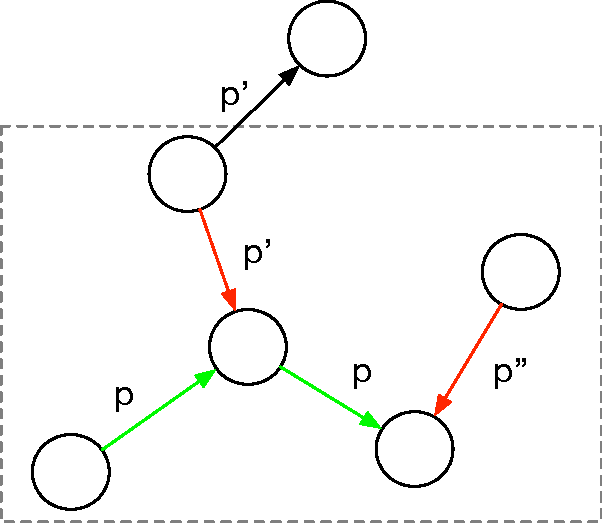
\includegraphics[width=0.4\linewidth]{figures/4_implementation/subgraph}
	\caption{Extraction of a sub graph (marked by dashed rectangle).}
	\label{fig:subgraph}
\end{figure}

There is another use case, in which sub graphs of a different kind are necessary. The results of Ch.~\ref{sec:evaluationHDTvsGRP} have also shown that GRP has a quite high run time even for smaller graphs. It was also mentioned in~\cite{maneth} that the rudimentary implementation (see Ch.~\ref{sec:relatedworkGRPImpl}) cannot handle very large graphs. However, we still want to evaluate GRP for real datasets which are often very large. To solve this problem, a realistic sub graph of the big graphs has to be extracted. As mentioned earlier, choosing random triples does not fulfill that. Hence, we choose an approach similar to the one shown in Fig.~\ref{fig:subgraph}. But here, we start with some entity $e$ (not with a set of desired properties). Analogously to the other approach, we gather all triples $e$ is part of. This gives us new entities $e_1,...,e_n$. Then, triples are added which $e_1,...,e_n$ are part of. That routine is repeated a few times, until some defined number of triples has been reached. 



\subsection{Dictionary Improvements}\label{sec:implementationDictImprovements}

For the dictionary improvements, HDT's dictionary compression (\DHDT{}) is used as a basis. Therefore, the HDT-Java code~\footnote{https://github.com/rdfhdt/hdt-java} has been extended.

\subsubsection{Literals}\label{sec:implementationLiterals}

As already mentioned in Ch.~\ref{sec:approachDictImprovements}, literals will be compressed using a Huffman code. To achieve that, HDT is changed such that it does not compress literals by prefix trees, but rather gives the literals to the newly created {\tt HuffmanHandler}, which compresses all literals and finally stores them in a binary format. In order to make that possible, the {\tt HuffmanHandler} has to traverse all literals in the beginning of the compression to establish a Huffman Tree.

In addition, the Huffman Tree itself has to be stored in order to be able to decompress the data. There is no standard way for storing the tree. One approach can be seen in Alg.~\ref{alg:HuffmanEncode}, which has to be started at the root node. That method creates an unambiguous bit representation of the tree. It traverses the tree in a depth-first-search-manner and writes a one (and the node's character) if the current node is a leaf. Otherwise, it writes a zero and the procedure is then called recursively for the current node's children. This encoding is unambiguous, because each node is either a leaf or has exactly two children.

\begin{algorithm}
	\caption{EncodeNode (TreeNode node)}\label{alg:HuffmanEncode}
	\begin{algorithmic}[1]
		\If{node is leaf}
		\State writeBit(1)
		\State writeCharacter(node.character)
		\Else
		\State writeBit(0)
		\State EncodeNode(node.leftChild)
		\State EncodeNode(node.rightChild)
		\EndIf
	\end{algorithmic}
\end{algorithm}


Alternatively, there are pre-computed Huffman trees for natural languages such as English. There, it has already been investigated which letter occurs how often in English texts and in this way a generally valid Huffman Tree has been established. The advantage is that the Huffman Tree does not have to be stored and it does not have to  be calculated, which saves runtime. The disadvantage, however, is that the tree is not optimal for the text to be compressed, as it is more general. Another problem in our case is that the literals contain a lot of special characters that are not taken into account in prefabricated Huffman Trees. Therefore, prefabricated trees will not be used.

\subsubsection{Blank Nodes}\label{sec:implementationBlankNodes}

HDT normally uses arbitrary and long strings generated by the Jena API and tries to compress them using prefix trees.

Thus, two approaches, which have both been implemented, for improving the compression of blank nodes are presented.

The first approach is to use shorter IDs (e.g. numbers from 1 to $n$). Then, during the run time a mapping from old ID to new ID is maintained by the new class {\tt BlankNodeHandler} in order to make sure that the same blank node will get the same new ID if it occurs multiple times. That mapping does not have to be stored persistently and will therefore be omitted once the compression is finished.

The second approach is to omit blank node IDs completely. The HDT code is changed in such a way that skips blank nodes in the process of storing the dictionary. HDT must then be changed so that it can handle the case in which it does not find a corresponding string in the dictionary for a certain short ID. At this point, it would know that the considered node is a blank node and the longer blank node ID is unimportant. Such a situation will occur when a decompression is performed. That mechanism has not been implemented, because this thesis is only interested in potential compression ratio improvements.

















